\documentclass{article}
\usepackage[hscale=0.7,vscale=0.8]{geometry}
\usepackage{lipsum}
\usepackage{graphicx}
\usepackage{amsmath}
\usepackage{verbatim}
\title{AG44 : Ski Resort}
\author{Guillaume OBERLE}
\date{9 December 2013}
\pagenumbering{gobble}
\begin{document}
\maketitle

\section{Introduction}
    \paragraph{}
        A director of a large ski resort of Savoie seeks to optimize the business management to make the ski area more attractive for the tourist. He wants to install kiosks in the ski queues and various points of the station which allow the skiers to choose their routes. He want to explain them how to travel to any other point of the resort as quickly as possible. 

\section{Data Structures}
    \paragraph{}
        The graph is represented by an object. It contains a list of nodes and a list of edges. Each nodes and edges is a tuple in the list and contains a dictionary for the attributes. Here is an example :
        \newline{}
        \newline{}
        An edge (1,2) : (1, 2, \{'color': 'grey', 'type': 'TS', 'weight': 600.0, 'label': 'replat'\})\\
        The type attribute define the type of the route.\\
        The weight attribute define the time in second to traverse this route.\\
        The label attribute define the name of the route.\\
        The color attribute is used to draw the graph.\\
        \newline{}
        A node (1) : (1, \{'altitude': 1200, 'label': 'villaroger'\})\\
        The altitude attribute define the altitude of the place.\\
        The label attribute define the name of the place.

\section{Algorithms}
    \paragraph{}
        To determine the shortest path, I have used the Floyd Warshall algorithm. I choose this algorithm because we have no negative cycle. Moreover, this software may be installed in a kiosk, and I think it's more efficient to calculate the shortest path between all pairs of vertices at the beginning and reconstruct the path when a client ask it.
    \paragraph{}
        To determine the reachable points according to the level of the skier, I used the Depth First Search algorithm. I had to modify it a little bit to handle the level of the skier but it work's fine. 
\newpage{}
\section{Example}
    \paragraph{}
        Here is an example for the shortest path between 1 and 4 and the reachable points from node 31 with only green routes.
    \paragraph{}
        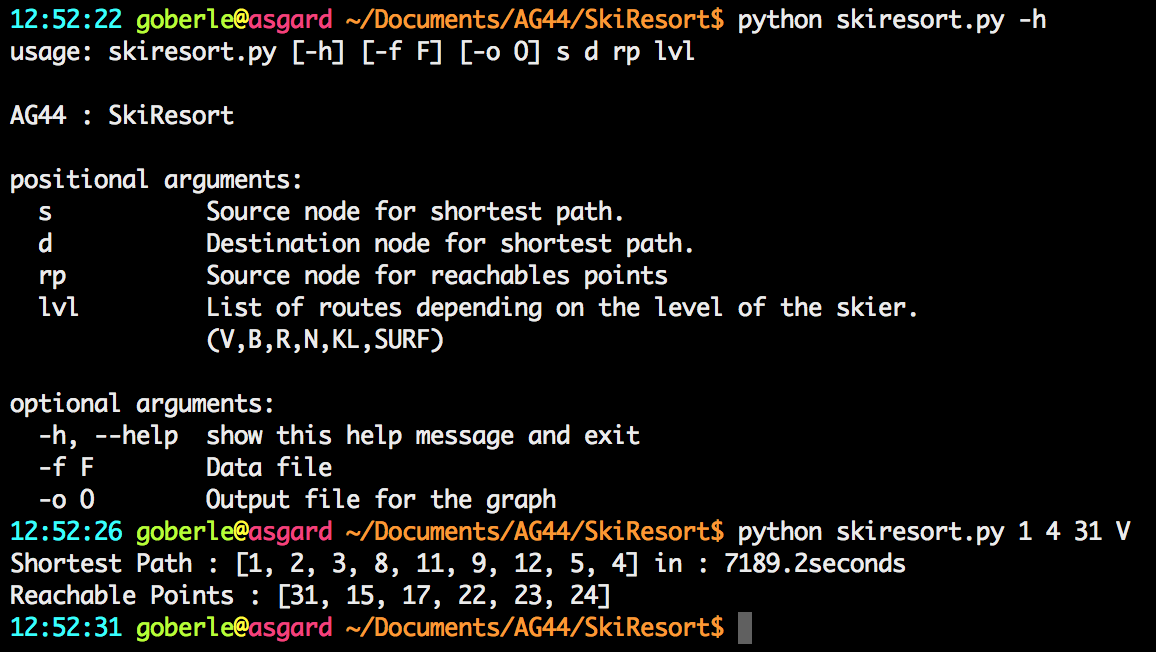
\includegraphics[scale=0.60]{example.png}

\section{Graph}
    \paragraph{}
        In order to have a big picture of what's the routes look like, I have done a Graph with the graphviz library. For the shortestpath, nodes fontcolor are in red and their edges are heavier and for the rechable points problem, the start node is in green and the reachable points are in grey. Here is a screenshot of the graph : 
    \paragraph{}
        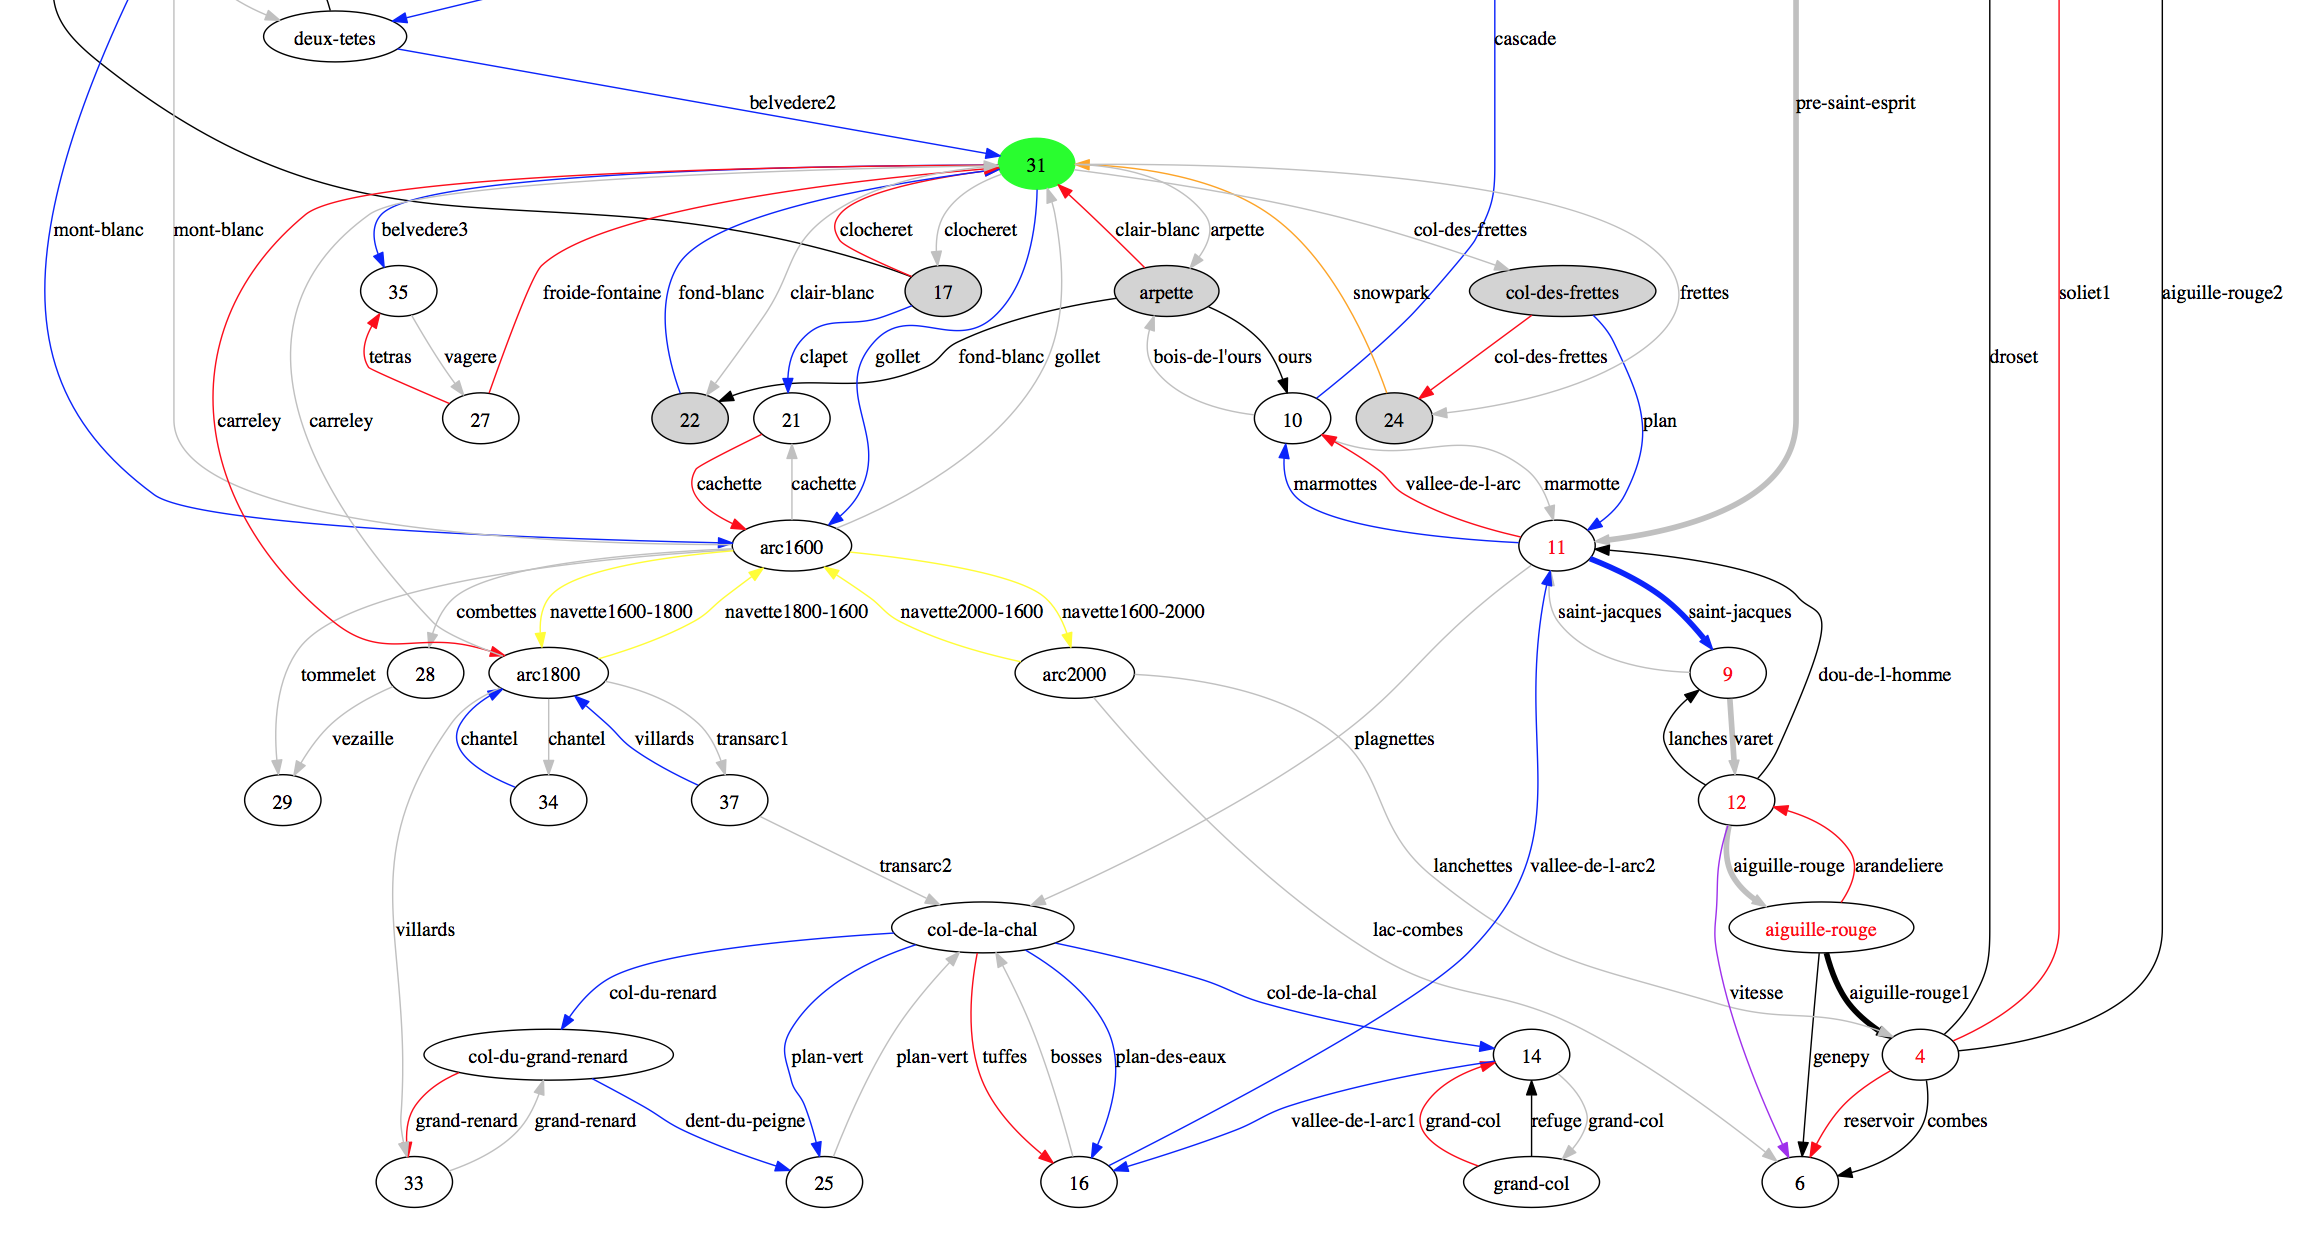
\includegraphics[scale=0.43]{example2.png}

\end{document}